%	Copyright (C) 2013 Systems Engineering Group
%
%	CHANGELOG:
%       2005-10-10 - corrected and extended. 
%       2013-01-28 - adjusted sections and explanation
%


\documentclass[a4paper,10pt,twoside]{article}
\usepackage{blindtext}
\pagestyle{headings}
\usepackage{a4wide}
\usepackage{graphicx}
\usepackage[font=small,labelfont=bf]{caption}
\usepackage{caption}
\usepackage{subcaption}
\usepackage[colorlinks,hyperfigures,backref,bookmarks,draft=false]{hyperref}

\title{Sudokount}
%\author{John Doe\\Magic Department, Richard Miles University}
\author{Ansh Rupani \\ \\ \\Matrikel. Nr: 4676365 \\ \\ \\Study Program: Master of Science in Distributed Systems Engineering \\ \\ \\Email: ansh.rupani@tu-dresden.de}
\date{\today}

\begin{document}

\maketitle


%\begin{abstract}
%There has been an ever growing demand of multi-core architectures for achieving higher levels of concurrency. Multi-threaded programing faces new challenges on throughput-oriented architectures like GPUs. The immense performance pressure on synchronization primitives like mutexes on tasks like memory allocation is unimaginable due to the extremely high number of threads in such architectures. The authors in \cite{gelado2019throughput} propose various concurrent programming techniques for GPU architectures to support better dynamic memory allocation.
%
%The authors have build their memory allocator with the support of other improvements they have proposed in the paper. They have proposed bulk semaphores, a generalized variant of counting semaphores which supports the case when multiple threads operate on a semaphore concurrently. A better approach for synchronization mechanisms like Read-Copy-Update has been proposed where multiple threads are allowed to access the critical section of the program simultaneously. Also, techniques to delegate deferred reclamation to threads which are already blocked have been proposed. All these proposed techniques when combined together contribute towards a highly throughput-oriented GPU memory allocator, which performs 16.56 times better than the CUDA based memory allocator in terms of allocation rates.
%\end{abstract}

\pagebreak

\tableofcontents

\newpage

\section{Problem Description}

The problem being discussed in this report is the \textit{Sudokount} problem. Sudoku is a puzzle which normally has a grid with dimensions 9 X 9. Internally, this grid is divided into 9 symmetrical square boxes, containing 9 elements each. Obviously, this grid has 9 rows and 9 columns. In the usual puzzle, some of these rows, columns and boxes are filled with digits 1 to 9. Completing the rest of the grid is the puzzle, however, it is not easy due to some constraints defining the way the grid can be filled. The grid elements should be filled up in such a way that that no column, row or box has any of the digits repeated.

Coming to the current task, the sudokount code calculates the number of possible solutions for a given input sudoku grid of any N X N dimensions (in the above example, N = 9). 

\section{In Depth Analysis of the Unoptimized Algorithm}
The provided sequential solution is based on the sudoku solving algorithm proposed by Peter Norvig \cite{norvig}. It is based on two basic ideas of constraint propagation and search.\\ \\
The terminology used by him is as follows:\\
1) A Sudoku puzzle is a \textit{grid} of 81 \textit{squares}.\\
2) A \textit{unit} is a collection of nine \textit{squares} (\textit{column}, \textit{row}, or \textit{box}).\\
3) \textit{Peers} are the \textit{squares} that share a \textit{unit}.\\
Figure 1 shows a 9 X 9 sudoku puzzle  with the used terminology for reference.\\ \\

\begin{figure}[h]
	\centering
	\scalebox{0.5}{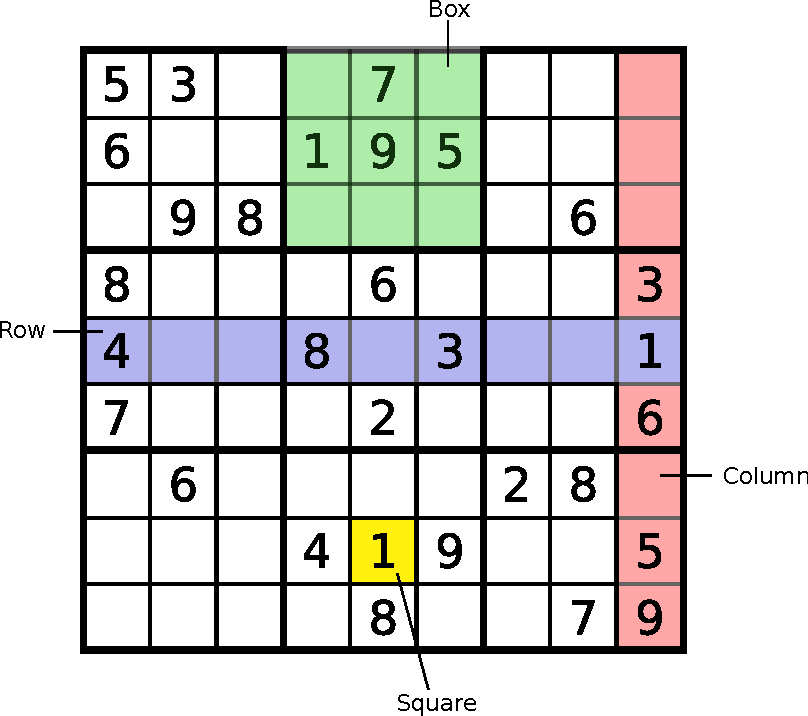
\includegraphics[width= \linewidth]{paper/sudoku}}
	\caption{Sudoku Puzzle}
	\label{fig:ualloc}
\end{figure}
According to his algorithm:\\
``\textit{A puzzle is solved if the squares in each unit are filled with a permutation of the digits 1 to 9.}"\\ \\
By this, it means that no digit can appear twice in a unit, however every digit must appear once. This means that each square must not have a value that is also the value of any of its peers.\\
The provided code first takes the number \textit{n} as input (for dimensions N X N where N = $n^{2}$) along with the grid.\\ \\
Then, a method \textit{create\_sudoku} is called which creates the sudoku puzzle and initializes it basically for the remainder of the code to work on. Different \textit{Structs} manage the values in a cell or square (\textit{cell\_v}), the coordinates (\textit{cell\_coord}) and the puzzle itself (\textit{sudoku}).\\ \\
An interesting choice has been made for the data structure used for the cell values (\textit{cell\_val}), which functions as a \textit{bitarray}, making it easier to eliminate the unnecessary choices for the \textit{squares} and further handle the puzzle in an intelligent manner. Thereafter, the \textit{init} function is called which initializes the respective coordinate structure for the unit lists and the peers. After this, the \textit{parse\_grid} function is called which sets the bit in the bitarray respective to the possible values of the square.Then, the \textit{assign} method is called which calls the \textit{eliminate} function to eliminate the values which are not possible for that particular square, also from the peers.\\ \\
The \textit{assign} and \textit{eliminate} basically take care of the constraint propagation part of the logic as well. The constraints defined by Norvig are as follows: \\
1) \textit{If a square has only one possible value, then eliminate that value from the square's peers.}\\
2) \textit{If a unit has only one possible place for a value, then put the value there.}\\ \\
The main algorithm starts with the \textbf{\textit{search}} function.
This function is called recursively until all possible favorable solution counts are accumulated.\\
The algorithm starts by choosing one unfilled square and consider all its possible values for the square. One by one, it assigns a possible value to the square and starts another search with this particular regard. This way, the \textit{search} method ``searches" for a value of a square such that a successful search could be initiated for a solution from the process of assigning this particular value to the particular square. In case the search operation results in a failure, the other value possible for the square should be considered. This is a recursive search in a depth-first search manner.\\ \\
According to Norvig:\\ \\
``\textit{To avoid bookkeeping complications, we create a new copy of values for each recursive call to search. This way each branch of the search tree is independent, and doesn't confuse another branch}".\\ \\
This is an important fact which is further exploited for parallelism. This algorithm is used as-is for the parallelism task, because it is highly optimized it offers task independency.

\section{Complexity Analysis}
For the part before calling the \textit{solve} or \textit{search} operations, i.e. the creation part, in the \textit{init} method, the loops have a complexity of $O(N^{3})$ at least. Further, the complexity of the recursive search algorithm increases enormously with an increase in the dimensions of the sudoku as it incorporates various loops as well.

\section{Parallelization Strategies}


\subsection{Parallelizing the \textit{search} Operation}
Exploiting the fact that Norvig stated in his blog, that each branch of the search tree is independent and does not interfere with another branch, is the key here\cite{chiu2012}.\\ \\
Before venturing into more explanation on why the \textit{search} operation was parallelized, it is important to analyze why the constraint propagation part of the algorithm \textit{should} not be parallelized. This analysis is important because constraint propagation (handled by the \textit{assign} and \textit{eliminate} functions) also consumes decent amount of time, since each search call initiates a call to \textit{assign} which further propagates to \textit{eliminate}.\\ \\
The reason is that there are various interdependencies when it comes to this part of the algorithm being parallelized. Suppose a particular thread modifies the possible values list for a particular square at this stage, the other threads running concurrently would have to be stalled until they receive this information. This would become a bottleneck again and again and cause a degrade of performance rather than improving the performance.\\ \\
Therefore, this directly implies that parallelizing the \textit{search} operation would be a better option. By doing this, we will allow various threads to solve the sudoku puzzle at the same time without interfering with each other. As soon as a thread finds a solution, it
can update the solution count. If not for multi-threaded implementation, a single thread would have to analyze all these possibilities one by one, making the algorithm slower as opposed to its capacity. Thus, its makes the best sense to allow individual threads handle individual branches parallely. This also highlights the concepts of \textbf{\textit{task parallelism}}, where the operations involved in arriving at the solution are distributed across cores.\\ \\
In this process, there were three important decisions involved: \\
1) \textbf{Overhead by threads}- \textit{The use of threadpool}: To avoid the overhead incurred by creating and joining threads everytime a \textit{search} call is made, threadpool has been used. This choice helps in reducing such overhead by creating all possible threads at once, and then queuing up the tasks while other tasks are being handled, with a promise of handling them next if they are next in the queue. \\ \\
2) \textbf{Use of synchronization barriers}- \textit{Global solution counter with lock}: Since various threads will be competing to update the solution count value, it makes sense to see it as a critical section of the algorithm. Therefore, since many threads try to update it at the same time this particular part is protected by a mutex lock.\\ \\
3) \textbf{Load analysis}- \textit{Allowing threads to go until a particular task depth}: To prevent overloading individual threads from going down a particular branch of the recursive algorithm, which might have a huge depth, it makes sense to put another thread to work by adding the appropriate task to the threadpool.
\subsection{Parallelizing the \textit{init} Operation}
Even though the \textit{init} method is called once, due the the high complexity involved in the operation for initializing the unit lists and peers, an opportunity exists to parallelize the working of the inner loops and handle the $O(kN)^{3}$ complexity. These tasks are independent of each other and therefore provide a parallelization opportunity that can be seized. This is true for the peers as well as the unit lists. Another point that can be noted is that the threadpool initialized in the \textit{main} function will remain idle until the search operation is called after the invocation of the \textit{solve} method. To utilize it at this point of time, parallelization of the \textit{init} operation makes sense. This also highlights the concepts of \textbf{\textit{data parallelism}}, as the loop operations are parallelized to access individual elements of the data structures independently.

\subsection{Experimenting With Various Task Depths}
Peter Norvig claimed in his blog that for hard sudoku puzzles, an average of 64 possibilities need to be checked by searching through not more than 16 squares to get one particular solution for dimensions of 9 X 9, based on the data collected by solving 95 hard puzzles. This also suggests that if the overall possibilities for solving the puzzle exactly is 64, inclusive of the checking of an average of 16 squares, the actual depth that a thread goes to in search of a solution must not be a lot. Therefore, various task depths have been considered to observe the effect of this choice. Detailed discussions are presented in Section 5.

\subsection{Experimenting With Golang}
To exploit the fact that \textit{goroutines} are lighter than threads, an attempt was made to convert the current code to golang. Goroutines are lighter because they have faster startup time than threads. Also, they have built-in primitives for safer communication between themselves, using channels. Two separate codes were written- the first one was just the sequential implementation and the second one was a parallel implementation with goroutines and channels. However, there was in issue because of which the executable took too long to evaluate the output for box dimensions of more than 3. The same was the case for the parallelized version. The reason was the way of accessing the bitarray implementation in golang. It required 3 nested loops which looped for `N' times each (complexity of $O(N^{3})$), inside the \textit{search} call, which exploded the time, especially for larger Ns. Therefore, this code was not used for evaluation, however, it is available on github.





\begin{figure}[t]
	\centering
	\scalebox{1}{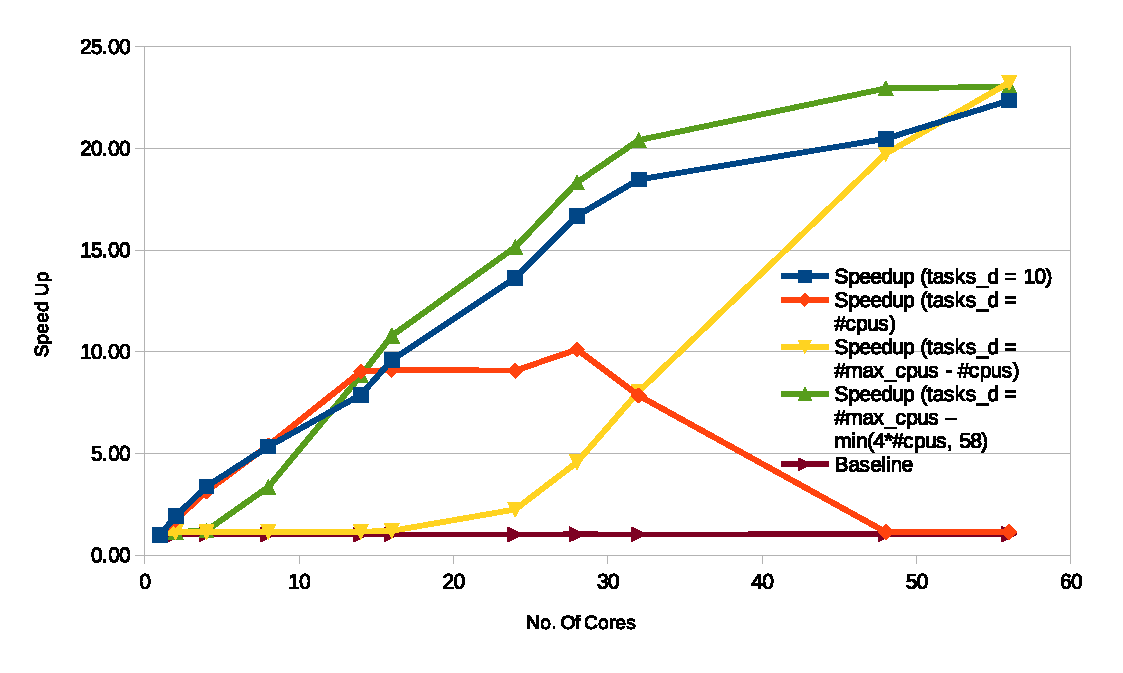
\includegraphics[width= \linewidth]{paper/graph.eps}}
	\caption{Speed Up For Various Strategies}
	\label{fig:ualloc}
\end{figure}

\section{Comparison and Evaluation}
Figure 2 and Figure 3 show the speed up and execution time respectively for various strategies.\\ \\
The factor to be compared is the variable \textit{tasks\_d}, which refers to tasks depth, which in turn signifies the depth of the search tree a particular thread would go. Experimentations were done with tasks depth of 10, \textit{cpus}, (\textit{CPUS\_MAX\_LIMIT} - \textit{cpus}) and (\textit{CPUS\_MAX\_LIMIT} - \textit{min(4*cpus, 58)}), where \textit{CPUS\_MAX\_LIMIT} and \textit{cpus} refer to the maximum number of cpus(or threads in the threadpool) that can be possible and the actual number of cores (or threads in threadpool) available. \\ \\
It was observed that the best results were obtained when tasks depth is decreased empirically with the increasing number of cores upto a certain limit, particularly the case where \textit{tasks\_d} = (\textit{CPUS\_MAX\_LIMIT} - \textit{min(4*cpus, 58)}). The reason behind this is that the workload is more optimally shared amongst the threads as more threads are available, without considering the waiting queue of the threadpool, as would have been the case with less number of cores and less task depths. However, in the third strategy, when the number of cores are less, the speed up observed is not decent enough. The reason behind this is the formula used for deciding the task depth, which does not seem suitable for linear or near linear scalability, however, after a certain number of cores (24), the curve is very much linear. In the fourth strategy, where  \textit{tasks\_d} = (\textit{CPUS\_MAX\_LIMIT} - \textit{min(4*cpus, 58)}), the distribution of tasks has been done empirically, better results are shown. The first strategy where the tasks depth is fixed to 10 also seems promising, because it maintains a lower depth in case of higher thread count, unlike the second strategy, where the tasks depth equals the number of cpus, which increases the depth with an increase in cpu count, thereby over or under utilizing the thread capacity in case of less or more number of cpus respectively.\\ \\
If not for the bad accessing techniques of the bitarrays in golang, its performance should also have been good because of less overhead of thread implementation.


\begin{figure}[t]
	\centering
	\scalebox{1}{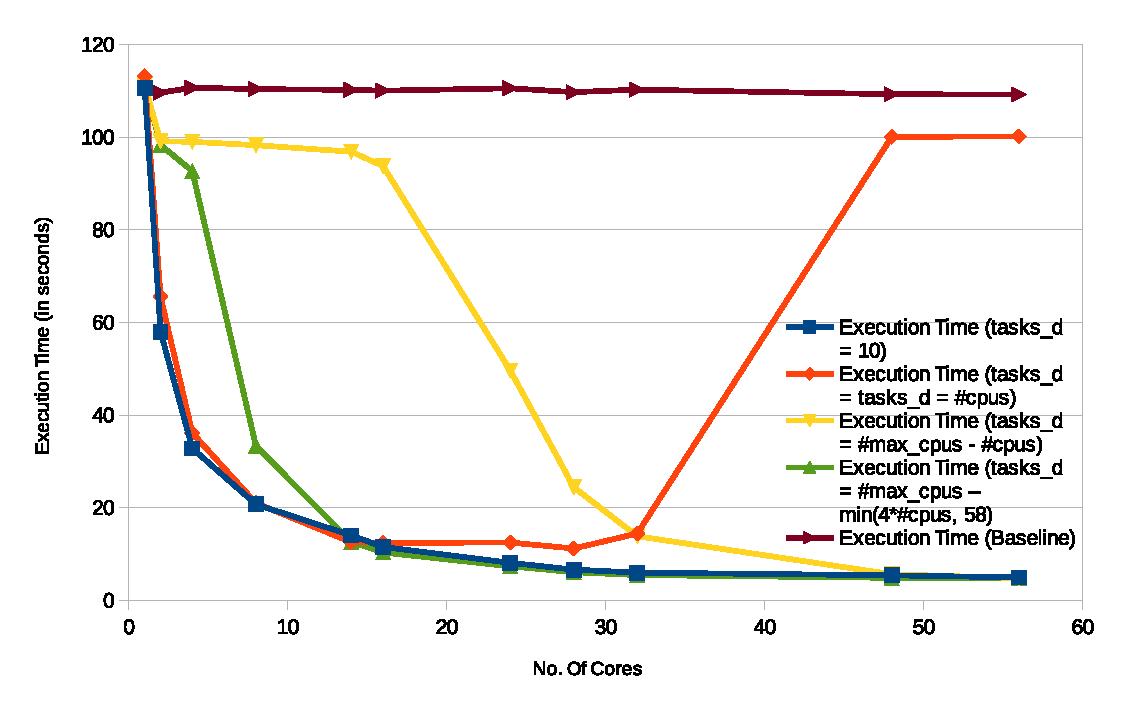
\includegraphics[width= \linewidth]{paper/execgraph.eps}}
	\caption{Execution Time For Various Strategies}
	\label{fig:ualloc}
\end{figure}

\section{Speed Up Discussion and Analysis of Amdahl's Law}
Amdahl's law states the maximum possible theoretical speed up for a task that can be attained by using all available cores. It suggests that the sequential part of the task limits the speed up. In Eq. (1), \textit{A} is the attainable speedup, \textit{p} is the fraction of the task that can be parallelized and \textit{n} is the number of cores. 
\begin{equation}
A = \frac{1}{(1-p) + p/n}
\end{equation}

Considering the baseline vs the version with \textit{tasks\_d} = (\textit{CPUS\_MAX\_LIMIT} - \textit{min(4*cpus, 58)}), the speed up is as follows: 

\begin{equation}
Speed~Up~_{28~cores} = \frac{111514379}{6076145} = 18.33
\end{equation}

\begin{equation}
Speed~Up~_{56~cores} = \frac{111514379}{4834080} = 23.04
\end{equation}

The speed up is nearly constant because of the reasons discussed above. However, using Eq. (1), following are the values for the parallel factor:

\begin{equation}
p~_{28~cores} =  0.98
\end{equation}

\begin{equation}
p~_{56~cores} =  0.97
\end{equation}


The \textit{p} values for 28 and 56 cores in Eq. (4) and (5), it can be seen that the values are similar, which normally is the case due to the cap in scalability infused by the sequential part of the task. These values attribute to the fact that the parallelization of any task is limited and restrained due to the sequential part.

\section{Appendix}

\begin{table}[h]
	\centering
	\scalebox{0.5}{\begin{tabular}{|l|l|l|}
			\hline
			\multicolumn{1}{|c|}{\textbf{Measurement}} & \multicolumn{1}{c|}{\textbf{Git Hash}} & \multicolumn{1}{c|}{\textbf{Evaluation URL}}                                                                                         \\ \hline
			Baseline                                   & cc67243                                & https://cds-lab-2019.netlify.com/logs/ef708123629f4ecf11cddda8fda3989645f7f572839455d588628a01a414a10b/2019-06-18T22:07:19+02:00.log \\ \hline
			tasks\_d = 10                              & b32760a                                & https://cds-lab-2019.netlify.com/logs/ef708123629f4ecf11cddda8fda3989645f7f572839455d588628a01a414a10b/2019-06-20T19:26:37+02:00.log \\ \hline
			tasks\_d = \#cpus                          & 558a65e                                & https://cds-lab-2019.netlify.com/logs/ef708123629f4ecf11cddda8fda3989645f7f572839455d588628a01a414a10b/2019-06-20T23:09:00+02:00.log \\ \hline
			tasks\_d = \#max\_cpus - \#cpus            & 282af19                                & https://cds-lab-2019.netlify.com/logs/ef708123629f4ecf11cddda8fda3989645f7f572839455d588628a01a414a10b/2019-06-21T13:54:13+02:00.log \\ \hline
			tasks\_d = \#max\_cpus – min(4*cpus, 58)   & 06a494e                                & https://cds-lab-2019.netlify.com/logs/ef708123629f4ecf11cddda8fda3989645f7f572839455d588628a01a414a10b/2019-06-21T18:38:29+02:00.log \\ \hline
		\end{tabular}}
	\end{table}

\bibliographystyle{alpha}
\bibliography{handin} 

\end{document}
